\documentclass[a4paper]{article}

\usepackage{fullpage} % Package to use full page
\usepackage{parskip} % Package to tweak paragraph skipping
\usepackage{tikz} % Package for drawing
\usepackage{amsmath}
\usepackage{siunitx} % Package for scientific units
\usepackage{amsfonts}
\usepackage{amssymb}
\usepackage{hyperref}
\usepackage[utf8]{inputenc}
\usepackage[english]{babel}
\usepackage{multicol}
\usepackage{graphicx} % Package for including images
\usepackage{mathtools}
\usepackage{pgfplots}
\graphicspath{ {./images/} }

\newcommand\tab[1][0.5cm]{\hspace*{#1}}
\DeclarePairedDelimiter\Floor\lfloor\rfloor
\DeclarePairedDelimiter\Ceil\lceil\rceil
\usepgfplotslibrary{polar}
\usepgflibrary{shapes.geometric}
\usetikzlibrary{calc}
\pgfplotsset{my style/.append style={axis x line=middle, axis y line=
middle, xlabel={$x$}, ylabel={$y$} }}
\pgfplotsset{compat=1.14}
\usepgfplotslibrary{fillbetween}


\title{Written Homework 1}
\author{Adrian Darian}
\date{1/25/2021}

\begin{document}
  
\maketitle
  
Complete the following tasks. You need to show work for full credit. In particular, for integrals, you may use resources like Wolfram Alpha to check your answers, but you need to show your work during Math 32 homework and exams. Some answers have been provided. Assemble your work into one PDF document and upload the PDF back into our CatCourses page.

\begin{itemize}
	\item[1.] Compute each of the following antiderivatives.
	      \begin{itemize}
	      	\item[(a)] $\int e^{-\frac{x}{32}} \,dx$ \\
	      	      \textbf{Answer:} 
	      	      \begin{equation}
	      	      	\begin{split}
	      	      		u = -\frac{x}{32} \\
	      	      		-32 \int e^u \,du \\
	      	      		-32 e^{u} \\
	      	      		-32 e^{\frac{x}{32}} + C \\
	      	      	\end{split}
	      	      \end{equation}
	      	\item[(b)] $\int xe^{-\frac{x}{32}} \,dx$ \\
	      	      \textbf{Answer:} 
	      	      \begin{equation}
	      	      	\begin{split}
	      	      		u = x, v' = e^{-\frac{x}{32}} \\
	      	      		-32xe^{-\frac{x}{32}} - \int -32e^{-\frac{x}{32}} \,dx \\
	      	      		-32xe^{-\frac{x}{32}} - 1024e^{-\frac{x}{32}} + C \\
	      	      	\end{split}
	      	      \end{equation}
	      	\item[(c)] $\int x^{2}e^{-\frac{x}{32}} \,dx$ \\
	      	      \textbf{Answer:} 
	      	      \begin{equation}
	      	      	\begin{split}
	      	      		u = x^{2}, v' = e^{-\frac{x}{32}} \\
	      	      		-32x^{2}e^{-\frac{x}{32}} - \int -64xe^{-\frac{x}{32}} \,dx \\
	      	      		-32x^{2}e^{-\frac{x}{32}} + 64(-32xe^{-\frac{x}{32}} - 1024e^{-\frac{x}{32}}) + C \\
	      	      	\end{split}
	      	      \end{equation}
	      \end{itemize} 
	\item[2.] Using your work from the previous problem, compute each of the following definite integrals.
	      \begin{itemize}
	      	\item[(a)] $\int_{0}^{\infty} e^{-\frac{x}{32}} \,dx$ \\
	      	      \textbf{Answer:} 
	      	      \begin{equation}
	      	      	\begin{split}
	      	      		-32 e^{\frac{x}{32}} + C \\
	      	      		\lim_{0\to\infty} (0 + 32) \\
	      	      		32 \\
	      	      	\end{split}
	      	      \end{equation}
	      	\item[(b)] $\int_{0}^{\infty} xe^{-\frac{x}{32}} \,dx$ \\
	      	      \textbf{Answer:} 
	      	      \begin{equation}
	      	      	\begin{split}
	      	      		-32xe^{-\frac{x}{32}} - 1024e^{-\frac{x}{32}} + C \\
	      	      		\lim_{0\to\infty} (0 - 1024 - \infty - \infty) \\
	      	      		1024 \\
	      	      	\end{split}
	      	      \end{equation}
	      	\item[(c)] $\int_{0}^{\infty} x^{2}e^{-\frac{x}{32}} \,dx$ \\
	      	      \textbf{Answer:} 
	      	      \begin{equation}
	      	      	\begin{split}
	      	      		-32x^{2}e^{-\frac{x}{32}} + 64(-32xe^{-\frac{x}{32}} - 1024e^{-\frac{x}{32}}) + C \\
	      	      		\lim_{0\to\infty} (0 + 64(0 - 1024) - \infty + 64(-\infty - \infty)) \\
	      	      		65536 \\
	      	      	\end{split}
	      	      \end{equation}
	      \end{itemize}  
	\item[3.] FizzBuzz and the Law of De Morgan In this setting, the universal set is the set of natural numbers from 1 to 32 \\
	      ${1, 2, 3, 4, \ldots, 32}$ \\
	      Let $T$ be the subset of numbers that are divisible by $3$ and let $F$ be the subset of numbers that are divisible by $5$.
	      \begin{itemize}
	      	\item[(a)] Write out lists of the elements of each of the following sets: $F, T, F^{c}, T^{c}$ \\
	      	      \textbf{Answer:} 
	      	      \begin{tabular}{rcl}
	      	      	$F$     & $=$ & $\{5, 10, 15, 20, 25, 30\}$                                                                          \\
	      	      	$T$     & $=$ & $\{3, 6, 9, 12, 15, 18, 21, 24, 27, 30\}$                                                            \\
	      	      	$F^{c}$ & $=$ & $\{1, 2, 3, 4, 6, 7, 8, 9, 11, 12, 13, 14, 16, 17, 18, 19, 21, 22, 23, 24, 26, 27, 28, 29, 31, 32\}$ \\
	      	      	$T^{c}$ & $=$ & $\{1, 2, 4, 5, 7, 8, 10, 11, 13, 14, 16, 17, 19, 20, 22, 23, 25, 26, 28, 29, 31, 32\}$               \\
	      	      \end{tabular}
	      	\item[(b)] We will do a "proof by example" of De Morgan's Law
	      	      \begin{itemize}
	      	      	\item[i.] Write out lists of the elements of $(F \cup T)^{c}$ \\
	      	      	      \textbf{Answer:}
	      	      	      \begin{equation}
	      	      	      	\begin{split}
	      	      	      		F = \{5, 10, 15, 20, 25, 30\} \\
	      	      	      		T = \{3, 6, 9, 12, 15, 18, 21, 24, 27, 30\} \\
	      	      	      		F \cup T = \{3, 5, 6, 9, 10, 12, 15, 18, 20, 21, 24, 25, 27, 30\} \\
	      	      	      		(F \cup T)^{c} = \{1, 2, 4, 7, 8, 11, 13, 14, 16, 17, 19, 22, 23, 26, 28, 29, 31, 32\} \\
	      	      	      	\end{split}
	      	      	      \end{equation}
	      	      	\item[ii.] Write out lists of elements of $F^{c} \cap T^{c}$ \\
	      	      	      \textbf{Answer:}
	      	      	      \begin{equation}
	      	      	      	\begin{split}
	      	      	      		F^{c} = \{1, 2, 3, 4, 6, 7, 8, 9, 11, 12, 13, 14, 16, 17, 18, 19, 21, 22, 23, 24, 26, 27, 28, 29, 31, 32\} \\
	      	      	      		T^{c} = \{1, 2, 4, 5, 7, 8, 10, 11, 13, 14, 16, 17, 19, 20, 22, 23, 25, 26, 28, 29, 31, 32\} \\
	      	      	      		F^{c} \cap T^{c} = \{1, 2, 4, 7, 8, 11, 13, 14, 16, 17, 19, 22, 23, 26, 28, 29, 31, 32\} \\
	      	      	      	\end{split}
	      	      	      \end{equation}
	      	      	\item[iii.] Make an observation about the previous two calculations \\
	      	      	      \textbf{Answer:} They are identical
	      	      \end{itemize}  
	      \end{itemize}
	\item[4.] The function $p(a)$ is defined for all real numbers $a$ as \\
	      \[
	      	p(a) =
	      	\begin{cases}
	      		1/36  & \text{, $a = 1$}   \\
	      		3/36  & \text{, $a = 2$}   \\
	      		5/36  & \text{, $a = 3$}   \\
	      		7/36  & \text{, $a = 4$}   \\
	      		9/36  & \text{, $a = 5$}   \\
	      		11/36 & \text{, $a = 6$}   \\
	      		0     & \text{, otherwise} \\
	      	\end{cases}
	      \] 
	      \begin{itemize}
	      	\item[(a)] Sketch the graph of the function $p(a)$. \\
	      	      \textbf{Answer:} 
	      	      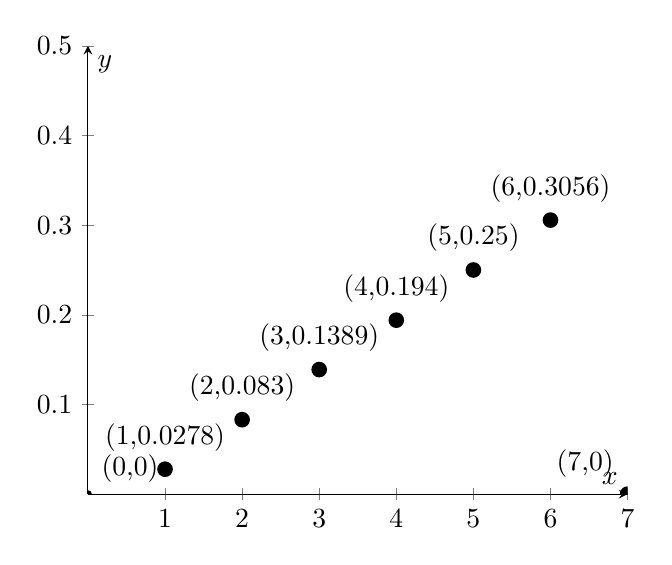
\begin{tikzpicture}
	      	      	\begin{axis}[my style,xtick={0,1,...,7},ytick={0,0.1,...,0.5},xmin=0,xmax=7,ymin=0,ymax=0.5]
	      	      		\node[label={30:{(0,0)}},circle,fill,inner sep=1pt] at (axis cs:0,0) {};
	      	      		\node[label={90:{(1,0.0278)}},circle,fill,inner sep=2pt] at (axis cs:1,0.0278) {};
	      	      		\node[label={90:{(2,0.083)}},circle,fill,inner sep=2pt] at (axis cs:2,0.083) {};
	      	      		\node[label={90:{(3,0.1389)}},circle,fill,inner sep=2pt] at (axis cs:3,0.1389) {};
	      	      		\node[label={90:{(4,0.194)}},circle,fill,inner sep=2pt] at (axis cs:4,0.194) {};
	      	      		\node[label={90:{(5,0.25)}},circle,fill,inner sep=2pt] at (axis cs:5,0.25) {};
	      	      		\node[label={90:{(6,0.3056)}},circle,fill,inner sep=2pt] at (axis cs:6,0.3056) {};
	      	      		\node[label={120:{(7,0)}},circle,fill,inner sep=2pt] at (axis cs:7,0) {};
	      	      	\end{axis}
	      	      \end{tikzpicture}
	      	\item[(b)] What are the values of $p(-0.5), p(0), p(2), p(3.5),$ and $p(7)$? \\
	      	      \textbf{Answer:} 
	      	      \begin{equation}
	      	      	\begin{split}
	      	      		p(-0.5) = 0 \\
	      	      		p(0) = 0 \\
	      	      		p(2) = 3/36 \\
	      	      		p(3.5) = 0 \\
	      	      		p(7) = 0 \\
	      	      	\end{split}
	      	      \end{equation}
	      \end{itemize}
	\item[5.] Consider the function $f(x)$ defined for all real numbers $x$ are \\
	      \[
	      	f(x) =
	      	\begin{cases}
	      		3/4 & \text{, $0 \leq x \leq 1$} \\
	      		1/8 & \text{, $2 \leq x \leq 4$} \\
	      		0   & \text{, otherwise}         \\
	      	\end{cases}
	      \] 
	      \begin{itemize}
	      	\item[(a)] Sketch the graph of $f$. \\
	      	      \textbf{Answer:} 
	      	      \begin{tikzpicture}
	      	      	\begin{axis}[my style,xtick={0,1,...,5},ytick={0,0.1,...,1},xmin=0,xmax=5,ymin=0,ymax=1]
	      	      		\addplot[domain=0:1,samples=5,thick] {3/4};
	      	      		\addplot[domain=1:2,samples=5,thick] {0};
	      	      		\addplot[domain=2:4,samples=5,thick] {1/8};
	      	      		\addplot[domain=4:5,samples=5,thick] {0};
	      	      	\end{axis}
	      	      \end{tikzpicture}
	      	\item[(b)] For each of the following definite integrals, sketch the graph with the correct area under the curve and compute the value.
	      	      \begin{itemize}
	      	      	\item[i.] $\int_{0}^{3} f(x) \,dx$ \\
	      	      	      \textbf{Answer:} 
	      	      	      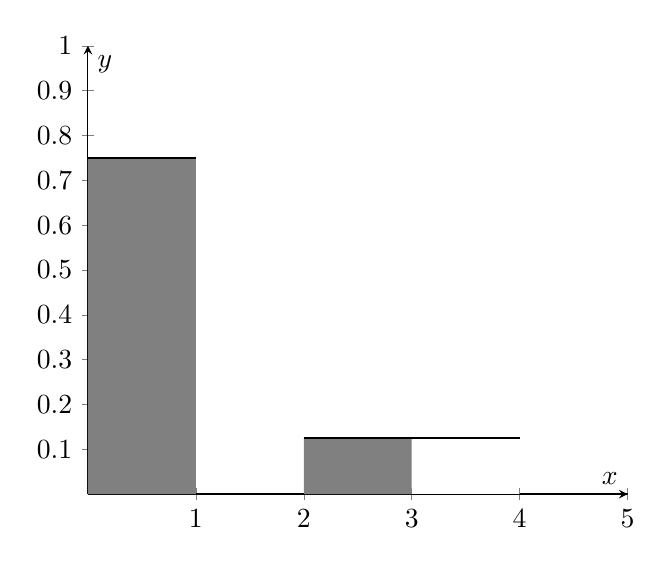
\begin{tikzpicture}
	      	      	      	\begin{axis}[my style,xtick={0,1,...,5},ytick={0,0.1,...,1},xmin=0,xmax=5,ymin=0,ymax=1]
	      	      	      		\addplot[domain=0:1,samples=5,thick,name path=A] {3/4};
	      	      	      		\addplot[draw=none,name path=B] {0};
	      	      	      		\addplot[domain=1:2,samples=5,thick] {0};
	      	      	      		\addplot[domain=2:4,samples=5,thick,name path=C] {1/8};
	      	      	      		\addplot[draw=none,name path=D] {0};
	      	      	      		\addplot[domain=4:5,samples=5,thick] {0};
	      	      	      		\addplot[gray] fill between[of=A and B,soft clip={domain=0:1}];
	      	      	      		\addplot[gray] fill between[of=C and D,soft clip={domain=2:3}];
	      	      	      	\end{axis}
	      	      	      \end{tikzpicture}
	      	      	      \begin{equation}
	      	      	      	\begin{split}
	      	      	      		\int_{0}^{3} f(x) \,dx \\
	      	      	      		\int_{0}^{1} \frac{3}{4} \,dx + \int_{1}^{2} 0 \,dx + \int_{2}^{3} \frac{1}{8} \,dx \\
	      	      	      		\frac{3}{4} \times (1 - 0) + 0 + \frac{1}{8} \times (3 - 2) \\
	      	      	      		\frac{7}{8} \\
	      	      	      	\end{split}
	      	      	      \end{equation}
	      	      	\item[ii.] $\int_{-\infty}^{1} f(x) \,dx$ \\
	      	      	      \textbf{Answer:} 
	      	      	      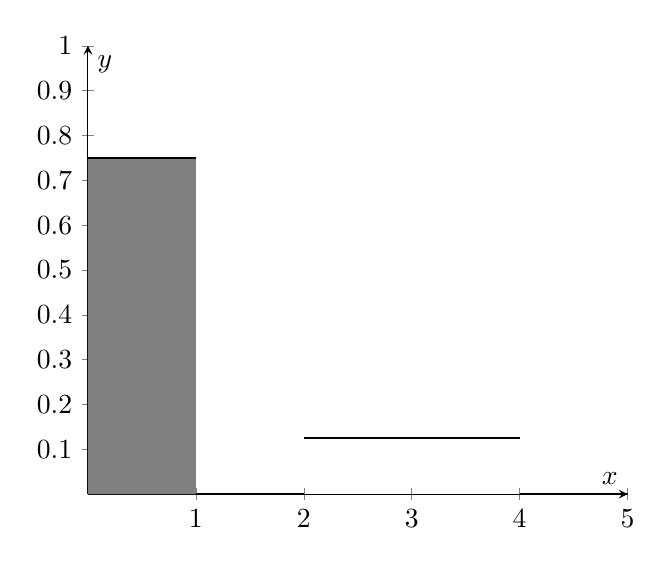
\begin{tikzpicture}
	      	      	      	\begin{axis}[my style,xtick={0,1,...,5},ytick={0,0.1,...,1},xmin=0,xmax=5,ymin=0,ymax=1]
	      	      	      		\addplot[domain=0:1,samples=5,thick,name path=A] {3/4};
	      	      	      		\addplot[draw=none,name path=B] {0};
	      	      	      		\addplot[domain=1:2,samples=5,thick] {0};
	      	      	      		\addplot[domain=2:4,samples=5,thick] {1/8};
	      	      	      		\addplot[domain=4:5,samples=5,thick] {0};
	      	      	      		\addplot[gray] fill between[of=A and B,soft clip={domain=0:1}];
	      	      	      	\end{axis}
	      	      	      \end{tikzpicture}
	      	      	      \begin{equation}
	      	      	      	\begin{split}
	      	      	      		\int_{-\infty}^{1} f(x) \,dx \\
	      	      	      		\int_{-\infty}^{0} 0 \,dx + \int_{0}^{1} \frac{3}{4} \,dx \\
	      	      	      		0 + \frac{3}{4} \times (1 - 0) \\
	      	      	      		\frac{3}{4} \\
	      	      	      	\end{split}
	      	      	      \end{equation}
	      	      	\item[iii.] $\int_{1.5}^{\infty} f(x) \,dx$ \\
	      	      	      \textbf{Answer:} 
	      	      	      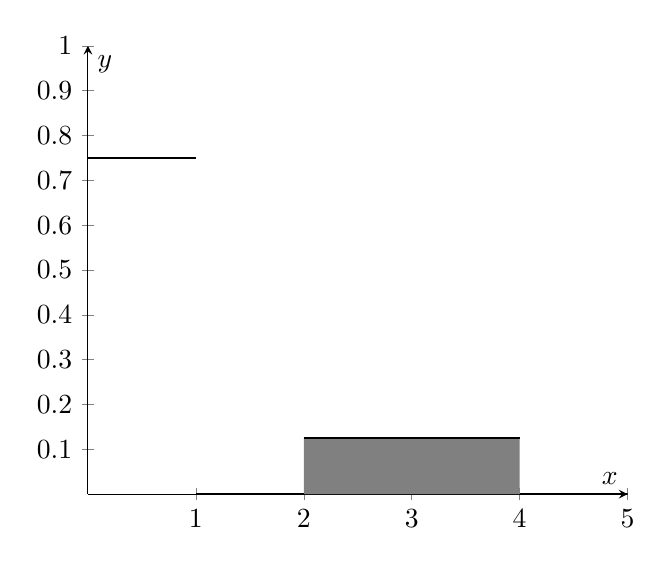
\begin{tikzpicture}
	      	      	      	\begin{axis}[my style,xtick={0,1,...,5},ytick={0,0.1,...,1},xmin=0,xmax=5,ymin=0,ymax=1]
	      	      	      		\addplot[domain=0:1,samples=5,thick] {3/4};
	      	      	      		\addplot[domain=1:2,samples=5,thick] {0};
	      	      	      		\addplot[domain=2:4,samples=5,thick,name path=A] {1/8};
	      	      	      		\addplot[draw=none,name path=B] {0};
	      	      	      		\addplot[domain=4:5,samples=5,thick] {0};
	      	      	      		\addplot[gray] fill between[of=A and B,soft clip={domain=2:4}];
	      	      	      	\end{axis}
	      	      	      \end{tikzpicture}
	      	      	      \begin{equation}
	      	      	      	\begin{split}
	      	      	      		\int_{1.5}^{\infty} f(x) \,dx \\
	      	      	      		\int_{1.5}^{2} 0 \,dx + \int_{2}^{4} \frac{1}{8} \,dx + \int_{4}^{\infty} 0 \,dx \\
	      	      	      		0 + \frac{1}{8} \times (4 - 2) + 0 \\
	      	      	      		\frac{1}{4} \\
	      	      	      	\end{split}
	      	      	      \end{equation}
	      	      \end{itemize}  
	      \end{itemize}
	\item[6.] Solve for x
	      \begin{equation}
	      	\frac{64}{3} = 16 \log_{\sqrt{x}} 64 + 8 \log_{\sqrt{x}} 64 + 4 \log_{\sqrt{x}} 64 + \ldots
	      \end{equation} \\
	      \textbf{Answer:}
	      \begin{equation}
	      	\begin{split}
	      		\frac{64}{3} = \log_{\sqrt{x}} 64 \times (16 + 8 + 4 + \ldots) \\
	      		1 = \log_{\sqrt{x}} 64 \times (16 + 8 + 4 + \ldots) \times \frac{3}{64} \\
	      		1 = \log_{\sqrt{x}} 64 \times (\frac{3}{4} + \frac{3}{8} + \frac{3}{16} + \ldots) \\
	      		1 = \log_{\sqrt{x}} 64 \times (1 + \frac{1}{2} + \frac{1}{4} + \ldots) \times \frac{3}{64} \\
	      		\sum_{i=0}^{\infty} \frac{1}{2}^{i} = \frac{1}{1 - \frac{1}{2}} = 2 \\
	      		1 = \log_{\sqrt{x}} 64 \times (\frac{3}{4}) \times 2 \\
	      		1 = \log_{\sqrt{x}} 64 \times (\frac{3}{2}) \\
	      		\frac{2}{3} = \log_{\sqrt{x}} 64 \\
	      		\sqrt{x}^{\frac{2}{3}} = 64 \\
	      		x = 262144 \\
	      	\end{split}
	      \end{equation}
	\item[7.] If you roll a pair of fair standard six sided dice, what is the probability that
	      \begin{itemize}
	      	\item[(a)] the sum is 7; \\
	      	      \textbf{Answer:} $\frac{3}{36} + \frac{3}{36} = \frac{6}{36}$
	      	\item[(b)] the larger number is at least 5: \\
	      	      \textbf{Answer:} $\frac{4}{6} \times \frac{5}{6} = \frac{20}{36}$
	      	\item[(c)] both numbers are at least 5? \\
	      	      \textbf{Answer:} $\frac{2}{36} + \frac{2}{36} = \frac{4}{36}$
	      \end{itemize}   
\end{itemize}

\end{document}